\documentclass{standalone}
\usepackage{tikz}
\usetikzlibrary{}
\usepackage{siunitx}
\begin{document}
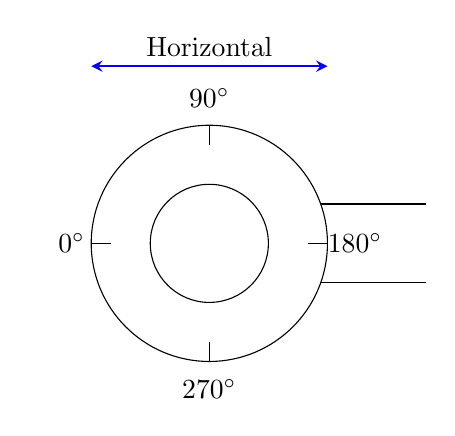
\begin{tikzpicture}
    
    \draw (0,0) circle (0.75);
    \draw (0,0) circle (1.5);
    \draw (1.25,0) -- (1.5,0);
    \draw (-1.25,0) -- (-1.5,0);
    \draw (0,1.25) -- (0,1.5);
    \draw (0,-1.25) -- (0,-1.5);
    
    \draw (1.42,0.5) -- (2.75,0.5);
    \draw (1.42,-0.5) -- (2.75,-0.5);
    
    \node at (-1.75,0) {\SI{0}{\degree}};
    \node at (0,1.85) {\SI{90}{\degree}};
    \node at (1.85,0) {\SI{180}{\degree}};
    \node at (0,-1.85) {\SI{270}{\degree}};
    
    \draw[<->, >=stealth, blue, thick] (-1.5,2.25) -- (1.5,2.25);
    \node at (0,2.5) {Horizontal};
    %\draw[<-, >=stealth, red, thick] (-2.15,0) arc (180:90:2.15);
    
    %\draw[fill=gray, fill opacity=0.8] (-1,1) -- (1,1) -- (1,-1) -- (-1,-1) -- (-1,1) ;
    %\draw[fill=gray, fill opacity=0.8] (-0.55,1.25) -- (-0.55,-1.25) arc (-90:90:1.25);
    %\draw[->, >=stealth, green, thick] (-0.35,0) -- (0.4,0);
    %\node[green] at (0,0.3) {Print};
    %\node[green] at (0,-0.20) {direc-};
    %\node[green] at (0,-0.50) {tion};
    
    % hack
    \draw[white] (-2.2,0) -- (-2.3,0);
\end{tikzpicture}
\end{document}